\chapter{Introducción}

A lo largo de este capítulo introduciremos los conceptos básicos sobre los que
vamos a trabajar.

% --- SECCIÓN ------------------------------------------------------------------
% --- TRANSFORMACIONES DE MÖBIUS -----------------------------------------------
\section{Transformaciones de Möbius}

Las transformaciones de Möbius poseen una dinámica sencilla de analizar. Por
esto, resultan un buen punto de partida para introducirse en la dinámica
compleja. Los ejemplos analizados en esta sección son algunos de los propuestos
en~\cite{Beardon1991}. Comencemos dando algunas definiciones y propiedades que
nos serán de utilidad.

\begin{definicion}
  Una transformación de Möbius es una función racional de la forma
  \begin{equation*}
    R(z) = \frac{az + b}{cz + d}, \quad ad-bc \neq 0,
  \end{equation*}
  donde $z$, $a$, $b$, $c$ y $d$ son números complejos.
\end{definicion}

Siguiendo los convenios habituales con el punto del infinito en la esfera de
Riemann, si $c \neq 0$: $R(\infty) = a/c$ y $R(-d/c) = \infty$. Si $c = 0$,
entonces, $R(\infty) = \infty$.

\begin{proposicion}
  Sea $R$ una transformación de Möbius distinta de la identidad. Entonces, $R$
  tiene dos puntos fijos, contando multiplicidades, en $\ExtC$.
\end{proposicion}
\begin{proof}
  Supongamos que $R(z) = (az + b)/(cz + d)$. Un punto $\zeta$ de $\ExtC$ es un
  punto fijo de $R$ si $R(\zeta) = \zeta$. Distinguimos tres casos:
  \begin{enumerate}[label=(\roman*)]
    \item si $c = 0$ y $a \neq d$, los puntos fijos son infinito y la solución
          de $(d-a)\zeta = b$; \label{itm:mobius_inf_fijo}
    \item si $c = 0$ y $a = d$, el infinito es un punto fijo doble; y
          \label{itm:mobius_inf_fijo_doble}
    \item si $c \neq 0$, los puntos fijos son las dos soluciones (contando
          multiplicidades) de $c\zeta^2 + (d - a)\zeta - b = 0$.\qedhere
  \end{enumerate}
\end{proof}

\begin{definicion}
  Sean $R$ y $S$ dos funciones racionales. Decimos que $R$ y $S$ son conjugadas
  si existe alguna transformación de Möbius $g$ tal que
  \begin{equation*}
    S = g R g^{-1}.
  \end{equation*}
\end{definicion}

La propiedad de ser conjugadas es una relación de equivalencia. Además, dos
funciones racionales conjugadas $R$ y $S$ cumplen las siguientes propiedades:
\begin{enumerate}[label=(\arabic*)]
  \item ambas funciones tienen el mismo grado;
  \item $S^n = g R^n g^{-1}$;
  \item un punto $\zeta$ es punto fijo de $R$ si y solo si $g(\zeta)$ lo es
        de~$S$; y
  \item un punto $z$ es periódico de periodo primo $n$ para $R$ si y solo si
        $g(z)$ lo es para $S$.
\end{enumerate}

En particular, $R^n=g^{-1}S^ng$. Como $g$ y $g^{-1}$ son continuas en la esfera
de Riemann, también podemos estudiar los límites de las órbitas de $R$ a partir
de los de $S$.

Existen otras definiciones de conjugación más generales. La que hemos tomado es
conocida como conjugación analítica o conforme, pero en dinámica compleja
también es habitual emplear conjugación topológica o conjugación cuasiconforme,
como se puede ver en~\cite{Beardon1991}.

\begin{proposicion}
  \label{prp:mobius_normal_form}
  Sea $R$ una transformación de Möbius distinta de la identidad. Entonces, $R$
  es conjugada a una función de una de las siguientes formas:
  \begin{enumerate}[label=(\arabic*)]
    \item $S(w) = w + 1$, si $R$ tiene un punto fijo con multiplicidad dos; o
    \item $S(w) = qw$, donde $q \in \C - \{0, 1\}$, si $R$ tiene dos puntos
          fijos diferentes.
  \end{enumerate}
\end{proposicion}
\begin{proof}
  Supongamos que $R$ tiene un único punto fijo $\zeta$ con multiplicidad dos.
  Primero, si $\zeta$ es finito, lo enviamos al infinito mediante la
  transformación de Möbius $g(z) = 1/(z - \zeta)$; si $\zeta=\infty$, tomamos
  $g$ igual a la identidad. La conjugada $S = g R g^{-1}$, que también es una
  transformación de Möbius, tiene como único punto fijo al infinito. Por tanto,
  es de la forma $w \mapsto aw + b$, con $a = 1$ por
  \ref{itm:mobius_inf_fijo_doble} de la demostración anterior, y $b \neq 0$
  (porque $R$ no es la identidad). Así $S(w) = w + b$, y conjugando con $h(w) =
  w/b$ tenemos que $R$ es conjugada a $w \mapsto w + 1$.

  Demostremos ahora el caso en que $R$ tiene dos puntos fijos diferentes,
  $\zeta_1$ y $\zeta_2$. En este caso enviaremos un punto fijo al cero y el
  otro al infinito. Si ambos puntos son finitos, utilizamos la transformación
  $g(z) = (z - \zeta_1)/(z - \zeta_2)$. Si uno de los dos ya es infinito,
  digamos $\zeta_2$, utilizaremos la transformación $g(z) = z - \zeta_1$. La
  transformación conjugada $S = g R g^{-1}$ fija el cero y el infinito, luego
  es de la forma $w \mapsto qw + b$, con $q \neq 0$. Como fija el cero, $b =
  0$, y como no es la identidad, $q \neq 1$. Concluimos así que $R$ es
  conjugada a $S(w) = qw$, con $q \in \C - \{0, 1\}$.
\end{proof}

Ilustremos cómo aplicar el procedimiento constructivo de la demostración
anterior mediante un par de ejemplos concretos.

\begin{ejemplo}
  \label{ej:mobius_iniciales}
  Consideremos
  \begin{equation}
    R_1(z) = \frac{3z - 2}{2z - 1} \quad \text{y} \quad R_2(z) = \frac{2z}{z+1}.
  \end{equation}
  Los puntos fijos de $R_1$ son las soluciones de la ecuación $z^2 - 2z +1 =
  0$, luego $\zeta = 1$ es su único punto fijo. Tomando $g_1(z) = 1/(z - 1)$,
  obtenemos que $R_1$ es conjugada a $S_1(w) = w + 2$. Por otro lado, $R_2$
  tiene dos puntos fijos distintos: $0$ y $1$. En este caso, escogiendo $g_2(z)
  = z/(z-1)$, obtenemos que $R_2$ es conjugada a $S_2(w) = 2w$.
\end{ejemplo}

Para describir la dinámica de estas transformaciones, será útil clasificar sus
puntos fijos según el comportamiento de las órbitas cercanas a ellos. Esta
clasificación se basa en el multiplicador, que introducimos a continuación.

\begin{definicion}
  Sea $R$ una función racional y $\zeta$ un punto fijo de $R$ en $\C$.
  Definimos el \emph{multiplicador} de $R$ en $\zeta$, denotado por
  $\multiplier{R}{\zeta}$, como el número complejo obtenido al evaluar la
  derivada en $\zeta$. Es decir,
  \begin{equation*}
    \multiplier{R}{\zeta} = R'(\zeta).
  \end{equation*}
\end{definicion}

El valor de la derivada en un punto fijo se conserva bajo conjugación, siempre
que tanto el punto fijo como su imagen sean finitos. En efecto, si $S = g R
g^{-1}$ y $R(\zeta) = \zeta$, la regla de la cadena da
\begin{equation*}
  S'(g(\zeta)) = g'(\zeta) R'(\zeta) (g^{-1})'(g(\zeta)) = R'(\zeta).
\end{equation*}
Esto nos permite extender la definición al caso en que $\infty$ sea un punto
fijo de $R$. Tomamos una transformación de Möbius $g$ tal que $g(\infty)$ sea
finito y definimos
\begin{equation*}
  \multiplier{R}{\infty} = \multiplier{g R g^{-1}}{g(\infty)}.
\end{equation*}
Esta definición no depende de la elección de $g$: dos elecciones se relacionan
mediante otra transformación de Möbius que conjuga los puntos fijos finitos
correspondientes, por lo que sus multiplicadores coinciden.

Antes de continuar con la clasificación, veamos intuitivamente por qué usamos
la derivada para caracterizar los puntos fijos. Si $\zeta$ es finito, el
desarrollo de Taylor da
\begin{equation*}
  R(z)-\zeta = R'(\zeta)(z-\zeta) + O(|z-\zeta|^2).
\end{equation*}
Así, si $|R'(\zeta)| < 1$, las distancias a $\zeta$ se contraen en un entorno
suficientemente pequeño y las órbitas que comienzan en él convergen a $\zeta$.
Si $|R'(\zeta)| > 1$, las distancias aumentan mientras las iteraciones
permanezcan en un entorno suficientemente pequeño. Cuando el multiplicador
tiene módulo $1$, el término lineal no basta, en general, para decidir el
comportamiento local. Para un punto fijo en el infinito, aplicamos el mismo
razonamiento tras enviarlo a un punto finito mediante una conjugación.

\begin{definicion}
  Sea $\zeta \in \ExtC$ un punto fijo de una función racional $R$. Entonces,
  $\zeta$ es:
  \begin{enumerate}[label=(\alph*)]
    \item \emph{superatractor} si $\multiplier{R}{\zeta} = 0$;
    \item \emph{atractor} si $0 < |\multiplier{R}{\zeta}| < 1$;
    \item \emph{repulsor} si $|\multiplier{R}{\zeta}| > 1$;
    \item \emph{racionalmente indiferente} si $\multiplier{R}{\zeta}$ es una
          raíz de la unidad; o \label{itm:racionalmente_indiferente}
    \item \emph{irracionalmente indiferente} si $|\multiplier{R}{\zeta}| = 1$,
          pero $\multiplier{R}{\zeta}$ no es una raíz de la unidad. \label{itm:irracionalmente_indiferente}
  \end{enumerate}
\end{definicion}

Habrá ocasiones en las que queramos referirnos tanto a puntos atractores como
superatractores; lo haremos diciendo que $\zeta$ es \emph{(super)atractor}. De
manera similar, diremos que $\zeta$ es \emph{indiferente} para referirnos tanto
a \ref{itm:racionalmente_indiferente} como a
\ref{itm:irracionalmente_indiferente}.

Gracias a la proposición~\ref{prp:mobius_normal_form} podemos ver que la
dinámica de las transformaciones de Möbius es tan sencilla como la de $w
\mapsto w + 1$ o $w \mapsto qw$. Esto nos va a permitir describir
explícitamente el comportamiento de las órbitas de todo $\ExtC$ bajo la acción
de una transformación de Möbius.

\begin{proposicion}
  \label{prp:dinamica_mobius}
  Sea $R$ una transformación de Möbius distinta de la identidad. Entonces, el
  comportamiento de las órbitas en $\ExtC$ queda completamente determinado
  según sus puntos fijos:
  \begin{enumerate}[label=(\arabic*)]
    \item Si $R$ tiene un único punto fijo $\zeta$, este es racionalmente
          indiferente (con multiplicador $1$) y $\lim_{n \to \infty} R^n(z_0) =
          \zeta$ para todo $z_0 \in \ExtC$.
    \item Si $R$ tiene dos puntos fijos distintos $\zeta_1$ y $\zeta_2$, se
          cumple exactamente uno de los siguientes casos para todo $z_0 \in
          \ExtC - \{\zeta_1, \zeta_2\}$:
          \begin{enumerate}[label=(\alph*)]
            \item Uno de los puntos fijos es atractor y el otro es repulsor, y
                  $R^n(z_0)$ converge al punto fijo atractor. \label{itm:mobius_dos_convergente}
            \item Ambos puntos fijos son racionalmente indiferentes, con
                  multiplicadores distintos de $1$, y todas las órbitas de
                  puntos no fijos tienen el mismo periodo primo.
            \item Ambos puntos fijos son irracionalmente indiferentes y la
                  órbita de $z_0$ es densa en una circunferencia o recta que
                  separa $\zeta_1$ y $\zeta_2$ en la esfera de Riemann. En el
                  caso de una recta, esta se entiende completada con el punto
                  del infinito.
          \end{enumerate}
  \end{enumerate}
\end{proposicion}
\begin{proof}
  Supongamos primero que $R$ tiene un único punto fijo $\zeta$. Por la
  proposición~\ref{prp:mobius_normal_form}, existe una transformación de Möbius
  $g$ con $g(\zeta) = \infty$ tal que $S = g R g^{-1}$ viene dada por $S(w) = w
  + 1$. Para calcular el multiplicador en $\infty$, conjugamos $S$ mediante
  $h(w) = 1/w$, obteniendo $h S h^{-1}(z) = z/(z+1)$, cuya derivada en $0$ es
  $1$. Por la invariancia del multiplicador bajo conjugación,
  $\multiplier{R}{\zeta} = \multiplier{S}{\infty} = 1$, por lo que $\zeta$ es
  racionalmente indiferente. Además, como $S^n(w) = w + n \to \infty$ para todo
  $w \in \ExtC$, concluimos por continuidad que $R^n(z_0) = g^{-1}(S^n(g(z_0)))
  \to g^{-1}(\infty) = \zeta$ para todo $z_0 \in \ExtC$.

  Supongamos ahora que $R$ tiene dos puntos fijos distintos, $\zeta_1$ y
  $\zeta_2$. Entonces, $R$ es conjugada a $S(w) = qw$ con $q \in \C - \{0, 1\}$
  mediante una transformación $g$ tal que $g(\zeta_1) = 0$ y $g(\zeta_2) =
  \infty$. Los multiplicadores de $S$ son $\multiplier{S}{0} = q$ y
  $\multiplier{S}{\infty} = 1/q$ (conjugando de nuevo con $w \mapsto 1/w$). Por
  invariancia, $\multiplier{R}{\zeta_1} = q$ y $\multiplier{R}{\zeta_2} = 1/q$.
  Como $S^n(w) = q^n w$, distinguimos según el módulo de $q$:
  \begin{itemize}
    \item Si $|q| \neq 1$, uno de los valores $|q|$ o $|1/q|$ es menor que $1$
          y el otro es mayor que $1$; por tanto, un punto fijo es atractor y el
          otro repulsor. Si $|q| < 1$, $S^n(w_0) \to 0$ para todo $w_0 \neq
          \infty$, luego $R^n(z_0) \to \zeta_1$. Análogamente, si $|q| > 1$,
          $S^n(w_0) \to \infty$ para todo $w_0 \neq 0$, luego $R^n(z_0) \to
          \zeta_2$. Esto prueba~\ref{itm:mobius_dos_convergente}.
    \item Si $|q| = 1$ y $q$ es una raíz de la unidad de orden $k \geq 2$,
          ambos puntos fijos son racionalmente indiferentes. Para cualquier
          $w_0 \in \C - \{0\}$, $S^n(w_0) = q^n w_0 = w_0$ si y solo si $k$
          divide a $n$, por lo que todo punto $z_0 \neq \zeta_1, \zeta_2$ es
          periódico de periodo primo $k$.
    \item Si $|q| = 1$ pero $q = e^{2\pi i \theta}$ con $\theta \in \R - \Q$,
          ambos puntos fijos son irracionalmente indiferentes. Por el teorema
          de aproximación de Kronecker, los múltiplos de $\theta$, considerados
          módulo $1$, son densos en $[0,1)$
          (véase~\cite[sección~7.4]{Apostol1990}). Por tanto, todo arco abierto
          de la circunferencia unidad contiene algún punto $e^{2\pi i
          n\theta}$, de modo que $\{e^{2\pi i n\theta} : n \geq 0\}$ es denso
          en ella. Por consiguiente, la órbita $\{S^n(w_0) : n \geq 0\}$ es
          densa en la circunferencia centrada en el origen de radio $|w_0|$.
          Dado que $g^{-1}$ es un homeomorfismo de $\ExtC$ que transforma
          circunferencias y rectas en circunferencias o rectas (circunferencias
          en sentido generalizado), la órbita $\{R^n(z_0) : n \geq 0\}$ es
          densa en la circunferencia o recta imagen por $g^{-1}$ de $|w| =
          |g(z_0)|$. Esta curva separa $\zeta_1$ y $\zeta_2$, pues la
          circunferencia original separa $0$ e $\infty$.\qedhere
  \end{itemize}
\end{proof}

Para concluir esta sección ilustraremos un ejemplo de cada caso.

\begin{ejemplo}
  Retomamos las transformaciones $R_1$ y $R_2$ del
  ejemplo~\ref{ej:mobius_iniciales}, junto con las funciones auxiliares $S_1$,
  $g_1$, $S_2$ y $g_2$.

  Para $R_1(z) = (3z-2)/(2z-1)$, su único punto fijo es $\zeta = 1$. Calculando
  su derivada obtenemos $R_1'(z) = 1/(2z-1)^2$, luego $\multiplier{R_1}{1} =
  1$, confirmando que $\zeta = 1$ es un punto fijo racionalmente indiferente.
  Puesto que es el único punto fijo, las órbitas de todos los puntos de $\ExtC$
  convergen a este. De hecho, desarrollando la composición $g_1^{-1} S_1^n g_1$
  (donde recordemos que $S_1(w) = w + 2$), obtenemos explícitamente
  \begin{equation*}
    R_1^n(z) = 1 + \frac{z - 1}{2n(z - 1) + 1},
  \end{equation*}
  y a partir de esta fórmula resulta inmediato comprobar que $\lim_{n \to
  \infty} R_1^n(z_0) = 1$ para todo $z_0 \in \ExtC$. En la
  figura~\ref{fig:mobius_iniciales} (izquierda) podemos ver las primeras
  iteraciones de un $z_0$.

  \begin{figure}[htbp]
    \centering
    \begin{subfigure}[b]{0.42\textwidth}
      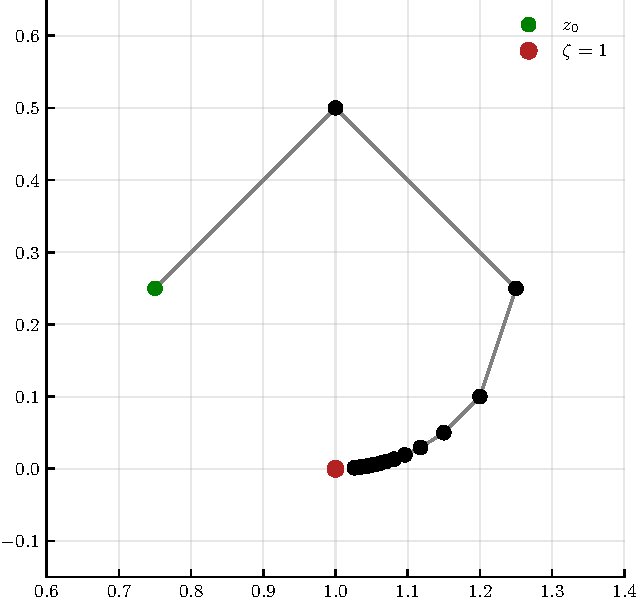
\includegraphics[width=0.9\textwidth]{mobius_one_fixed_point_orbit.pdf}
    \end{subfigure}
    \begin{subfigure}[b]{0.42\textwidth}
      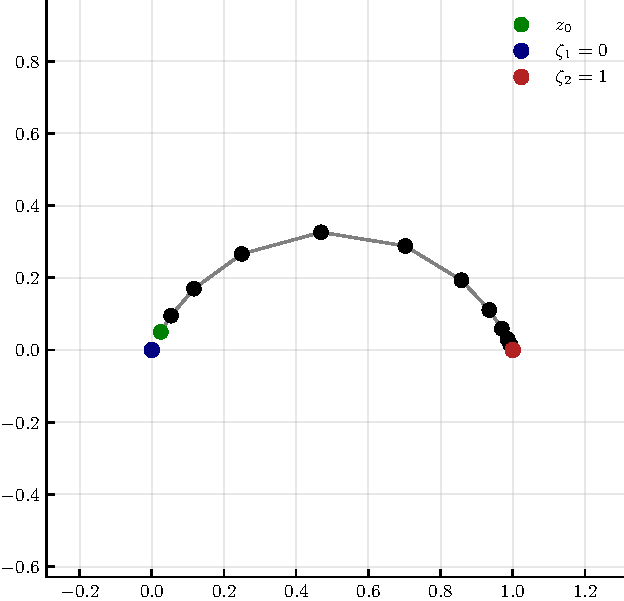
\includegraphics[width=0.9\textwidth]{mobius_two_fixed_points_convergent_orbit.pdf}
    \end{subfigure}
    \caption{El punto inicial $z_0$ está marcado en verde, en rojo el punto
             fijo al que converge la órbita y en azul el resto de puntos fijos.
             La gráfica de la izquierda muestra las primeras $20$ iteraciones
             de $R_1$ desde $(3 + i)/4$. La gráfica de la derecha muestra las
             primeras $10$ iteraciones de $R_2$ desde $(1 + 2i)/40$.}
    \label{fig:mobius_iniciales}
  \end{figure}

  Por otro lado, $R_2(z) = 2z/(z+1)$ es conjugada a $S_2(w) = 2w$ mediante
  $g_2(z) = z/(z-1)$, que envía $0$ a $0$ y $1$ a $\infty$. Como $R_2'(z) =
  2/(z+1)^2$, los multiplicadores son $\multiplier{R_2}{0} = 2$ y
  $\multiplier{R_2}{1} = 1/2$ (que coinciden con los de $S_2$ en $0$ e
  $\infty$, respectivamente). Por tanto, $0$ es un punto fijo repulsor y $1$ es
  un punto fijo atractor. Como $S_2^n(w) = 2^n w$, la órbita de cualquier $w_0
  \neq 0$ tiende a $\infty$. Traducido a $R_2$, esto significa que la órbita de
  cualquier $z_0 \neq 0$ converge al punto fijo atractor $g_2^{-1}(\infty) =
  1$, por muy cerca que tomemos $z_0$ del punto repulsor $0$ (véase la
  figura~\ref{fig:mobius_iniciales}, derecha).
\end{ejemplo}

Nos quedan por analizar el caso de órbitas periódicas y el de órbitas densas.
Comencemos con las órbitas periódicas.

\begin{ejemplo}
  Sea
  \begin{equation*}
    R(z)=\frac{(1+i)z+(1-i)}{(1-i)z+(1+i)}.
  \end{equation*}
  Sus puntos fijos son $1$ y $-1$. Con $g(z) = (z-1)/(z+1)$ se obtiene $S(w) =
  iw$. Los multiplicadores en $1$ y $-1$ son, respectivamente, $i$ y $-i$,
  luego ambos puntos son racionalmente indiferentes.

  Como $S^4(w) = w$, se tiene $R^4(z) = z$. Todo punto en $\ExtC$ es periódico,
  y los puntos no fijos tienen periodo primo $4$ (véase la
  figura~\ref{fig:mobius_periodica}). Esto se debe a que para $w \neq 0$,
  $\infty$ la igualdad $i^n w = w$ equivale a $i^n=1$.

  \begin{figure}[htbp]
    \centering
    \begin{subfigure}[b]{0.42\textwidth}
      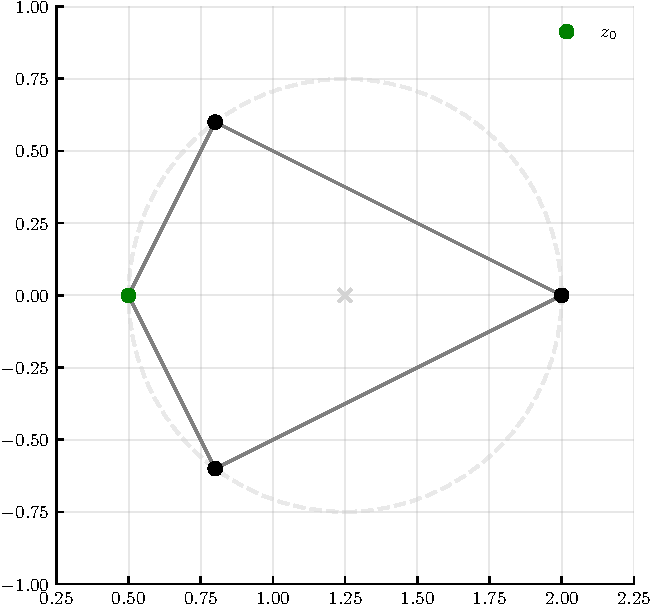
\includegraphics[width=0.9\textwidth]{mobius_two_fixed_points_periodic_orbit.pdf}
    \end{subfigure}
    \begin{subfigure}[b]{0.42\textwidth}
      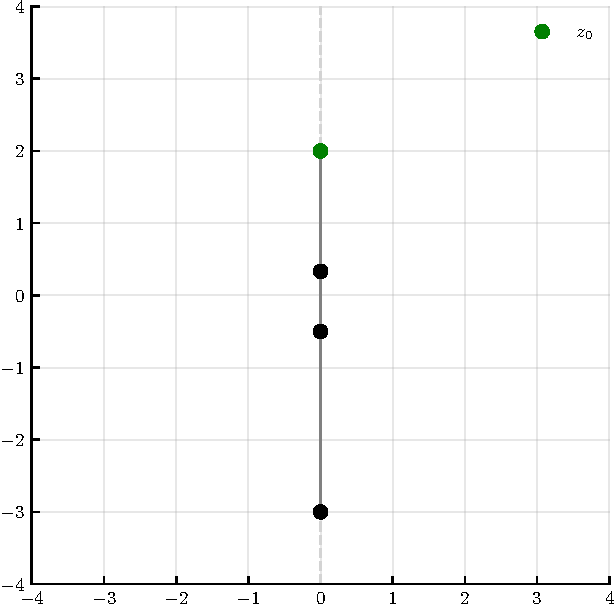
\includegraphics[width=0.9\textwidth]{mobius_two_fixed_points_periodic_orbit_imaginary_axis.pdf}
    \end{subfigure}
    \caption{Órbitas de los puntos $1/2$ y $2i$, de izquierda a derecha. En la
             gráfica de la izquierda se observa cómo todas las iteraciones
             pertenecen a la circunferencia dibujada. La gráfica de la derecha
             muestra un caso en el que en vez de una circunferencia, las
             iteraciones pertenecen a una recta.}
    \label{fig:mobius_periodica}
  \end{figure}

  Además, la órbita de un punto $z_0 \neq 1$, $-1$ está contenida en el
  conjunto
  \begin{equation*}
    \left|\frac{z-1}{z+1}\right|
    =\left|\frac{z_0-1}{z_0+1}\right|.
  \end{equation*}
  Estos conjuntos son circunferencias, salvo cuando $z_0$ se encuentra en el
  eje imaginario o es infinito, en cuyo caso se obtiene el eje imaginario junto
  con el infinito. Las fracciones anteriores son $g$ evaluada en $z$ y $z_0$;
  en particular, $g(\infty)=1$. Sea $k = |g(z_0)| > 0$ (pues $z_0 \neq 1, -1$).
  Los puntos $z \in \C$ de la órbita satisfacen $|z-1| = k|z+1|$. Elevando al
  cuadrado ambos miembros y escribiendo $z = x + iy$, obtenemos:
  \[
    (x-1)^2 + y^2 = k^2\big((x+1)^2 + y^2\big) \iff (1-k^2)(x^2+y^2) - 2(1+k^2)x + (1-k^2) = 0.
  \]
  Si $k = 1$, la ecuación se reduce a $-4x = 0$, que corresponde al eje
  imaginario $x = 0$ (junto con $\infty$). Para $z_0$ finito, esta condición
  equivale a $|z_0-1| = |z_0+1|$, es decir, a que $z_0$ equidiste de $1$ y
  $-1$; también se cumple cuando $z_0=\infty$.

  Si $k \neq 1$, podemos dividir entre $1-k^2$ y completar el cuadrado:
  \[
    \left(x - \frac{1+k^2}{1-k^2}\right)^2 + y^2 = \left(\frac{1+k^2}{1-k^2}\right)^2 - 1 = \left(\frac{2k}{|1-k^2|}\right)^2,
  \]
  lo que describe una circunferencia centrada en $\left(\frac{1+k^2}{1-k^2},
  0\right)$ y de radio $\frac{2k}{|1-k^2|}$.

\end{ejemplo}

\begin{observacion}
  Como curiosidad geométrica del ejemplo anterior, si tomamos un punto inicial
  racional $z_0 = p/q \in \Q$ (con $p, q \in \Z$ coprimos, $q \neq 0$ y $z_0
  \notin \{0,1,-1\}$), su segunda iteración es $z_2 = R^2(z_0) =
  g^{-1}(-g(z_0)) = 1/z_0$. Dado que el centro de la circunferencia invariante
  se encuentra en el eje real y tanto $z_0$ como $z_2$ son reales, los puntos
  $z_0$ y $z_2$ son los extremos de un diámetro de dicha circunferencia. Como
  $z_1 = R(z_0)$ también pertenece a la circunferencia, el teorema de Tales
  garantiza que el triángulo de vértices $z_0, z_1, z_2$ es rectángulo en
  $z_1$. Además, calculando la primera iteración obtenemos
  \begin{equation*}
    z_1 = \frac{2pq}{p^2+q^2} + i\frac{p^2-q^2}{p^2+q^2}.
  \end{equation*}
  Como $|z_1|=1$, resulta la identidad $(2pq)^2+(p^2-q^2)^2=(p^2+q^2)^2$, que
  proporciona la terna pitagórica $(|p^2-q^2|,2|pq|,p^2+q^2)$.
\end{observacion}

\begin{ejemplo}[Rotación irracional]
  Consideremos $R(z) = e^{2i} z$. Sus puntos fijos son $0$ e $\infty$, con
  multiplicadores $e^{2i}$ y $e^{-2i}$, ambos de módulo $1$. Si un punto $z
  \neq 0, \infty$ fuera periódico, existiría $n \geq 1$ tal que $e^{2ni} = 1$,
  es decir, $n = \pi k$ para algún entero $k$. Esto es imposible porque $\pi$
  es irracional. Como el ángulo de giro dividido por $2 \pi$ es el irracional
  $1 / \pi$, el teorema de aproximación de Kronecker muestra que cada una de
  estas órbitas es densa en la circunferencia $|w| = |z|$. En particular,
  permanece acotada, pero no converge.

  \begin{figure}[htbp]
    \centering
    \begin{subfigure}[b]{0.42\textwidth}
      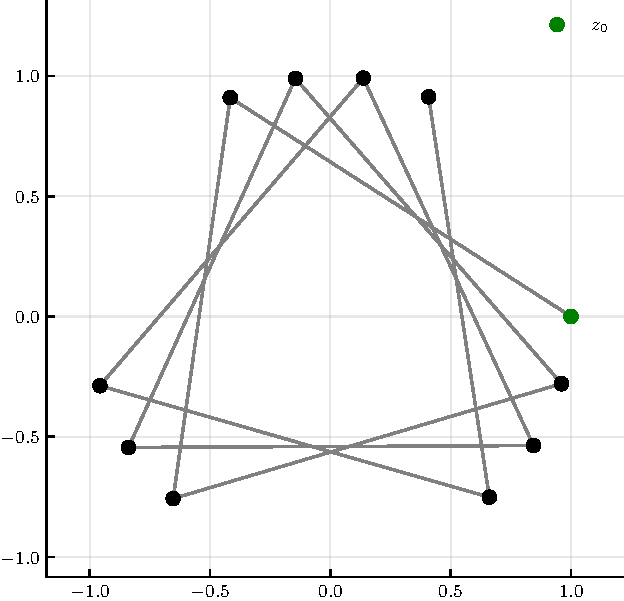
\includegraphics[width=0.9\textwidth]{mobius_two_fixed_points_dense_orbit_10.pdf}
    \end{subfigure}
    \begin{subfigure}[b]{0.42\textwidth}
      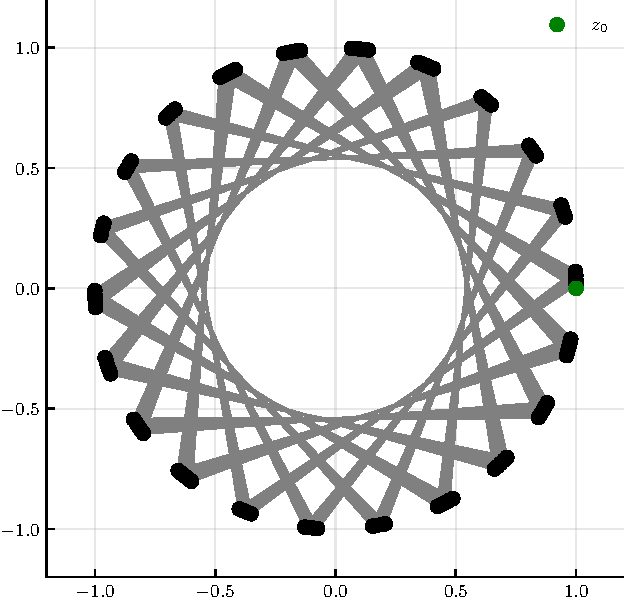
\includegraphics[width=0.9\textwidth]{mobius_two_fixed_points_dense_orbit_100.pdf}
    \end{subfigure}
    \caption{Primeras 10 y 100 iteraciones de $z_0 = 1$ mediante $e^{2i} z$.}
  \end{figure}
\end{ejemplo}

% En una transformación conjugada a una rotación irracional, las circunferencias
% anteriores se transportan mediante $g^{-1}$ a circunferencias o rectas
% completadas con el infinito. Por tanto, la conjugación permite describir tanto
% los límites y la periodicidad como los conjuntos geométricos que contienen las
% órbitas.
%
% % --- SECCIÓN ------------------------------------------------------------------
% % --- EL POLINOMIO z^2 ---------------------------------------------------------
% \section{El polinomio \texorpdfstring{$z^2$}{z cuadrado}}
% \label{sec:z_cuadrado}
%
% Consideremos ahora una función de grado dos,
% \begin{equation*}
%   R(z)=z^2.
% \end{equation*}
% Sus puntos fijos son $0$, $1$ e $\infty$. Como $R'(z)=2z$, el cero es
% superatractor y $1$ es repulsor. En el infinito, usando $u=1/z$,
% \begin{equation*}
%   \widetilde R(u)=\frac{1}{R(1/u)}=u^2,
% \end{equation*}
% de modo que el infinito también es superatractor. El análisis de este ejemplo
% aparece en~\cite[ejemplo~2, pp.~2--3]{Watanabe2003}; aquí estudiaremos primero
% sus órbitas, sin utilizar todavía la definición de los conjuntos de Fatou y de
% Julia.
%
% \subsection{Interior y exterior de la circunferencia unidad}
%
% Por inducción, para todo $n\geq0$ se tiene $R^n(z)=z^{2^n}$. Si escribimos
% $z=re^{i\theta}$, entonces
% \begin{equation*}
%   R^n(z)=r^{2^n}e^{i2^n\theta}.
% \end{equation*}
% En consecuencia,
% \begin{equation*}
%   R^n(z)\longrightarrow
%   \begin{cases}
%     0,      & |z|<1, \\
%     \infty, & |z|>1.
%   \end{cases}
% \end{equation*}
% Las cuencas de los dos puntos fijos superatractores son exactamente
% \begin{equation*}
%   A(0)=\{z\in\C:|z|<1\},\qquad
%   A(\infty)=\{z\in\C:|z|>1\}\cup\{\infty\}.
% \end{equation*}
% La convergencia al cero es uniforme en cada disco cerrado $|z|\leq r<1$, pues
% $|R^n(z)|\leq r^{2^n}\to0$. En el exterior, para $|z|\geq r>1$,
% \begin{equation*}
%   \sigma(R^n(z),\infty)
%   =\frac{1}{\sqrt{1+|z|^{2^{n+1}}}}
%   \leq\frac{1}{\sqrt{1+r^{2^{n+1}}}}\longrightarrow0.
% \end{equation*}
% Por tanto, también hay convergencia uniforme hacia el infinito en estas
% regiones, entendida en la métrica cordal.
%
% \subsection{Dinámica en la circunferencia unidad}
%
% Sea $C=\{z\in\C:|z|=1\}$. Como $|z^2|=1$ si y solo si $|z|=1$ y todo punto de
% $C$ tiene sus dos raíces cuadradas en $C$, se cumple $R(C)=C=R^{-1}(C)$. Es
% decir, tanto las imágenes como las preimágenes de $C$ permanecen en $C$.
%
% Escribiendo $z=e^{2\pi it}$, con $t\in[0,1)$, la aplicación restringida a $C$
% equivale a duplicar el ángulo módulo $1$:
% \begin{equation*}
%   e^{2\pi it}\longmapsto e^{2\pi i(2t)},\qquad
%   R^n(e^{2\pi it})=e^{2\pi i(2^nt)}.
% \end{equation*}
% Esto permite distinguir los siguientes comportamientos.
%
% \begin{ejemplo}[Puntos que llegan al punto fijo repulsor]
%   Un punto $z\in C$ llega a $1$ tras un número finito de iteraciones si y solo
%   si
%   \begin{equation*}
%     z=e^{2\pi ik/2^m},\qquad m\geq0,\quad 0\leq k<2^m.
%   \end{equation*}
%   En efecto, $R^m(z)=1$ equivale a $z^{2^m}=1$. Por ejemplo,
%   \begin{equation*}
%     e^{\pi i/4}\longmapsto i\longmapsto-1\longmapsto1.
%   \end{equation*}
%   Salvo $1$, estos puntos son eventualmente periódicos, pero no periódicos. Son
%   densos en $C$: para cada $m$ están uniformemente espaciados y la separación
%   angular $2\pi/2^m$ tiende a cero.
%
%   De hecho, no hay otras órbitas en $C$ que converjan a $1$. Para verlo,
%   escribamos $R^n(z)=e^{2\pi it_n}$, eligiendo $t_n\in[-1/2,1/2)$. Si
%   $R^n(z)\to1$, entonces $t_n\to0$. Para todo $n$ suficientemente grande,
%   $|t_n|<1/4$, por lo que $t_{n+1}=2t_n$ sin reducción módulo $1$. Esto solo
%   puede mantenerse si $t_n=0$ desde alguna iteración.
% \end{ejemplo}
%
% \begin{ejemplo}[Puntos periódicos]
%   Para $z\in C$ y $n\geq1$,
%   \begin{equation*}
%     R^n(z)=z\quad\Longleftrightarrow\quad z^{2^n-1}=1.
%   \end{equation*}
%   Por tanto, los puntos de $C$ cuyo periodo divide a $n$ son
%   \begin{equation*}
%     z=e^{2\pi ik/(2^n-1)},\qquad 0\leq k<2^n-1.
%   \end{equation*}
%   Hay órbitas de cualquier periodo primo $n\geq2$: basta tomar $z_n=e^{2\pi
%   i/(2^n-1)}$. En efecto, si $1\leq j<n$, entonces $0<2^j-1<2^n-1$, luego
%   $z_n^{2^j-1}\neq1$. Por ejemplo, para $n=2$ obtenemos
%   \begin{equation*}
%     e^{2\pi i/3}\longmapsto e^{4\pi i/3}\longmapsto e^{2\pi i/3}.
%   \end{equation*}
%   El conjunto de todos los puntos periódicos también es denso en $C$, porque la
%   separación angular $2\pi/(2^n-1)$ tiende a cero.
%
%   Además, todos estos puntos periódicos son repulsores para la iterada
%   correspondiente. Si $R^n(z)=z$ y $z\in C$, entonces
%   \begin{equation*}
%     (R^n)'(z)=2^n z^{2^n-1}=2^n>1.
%   \end{equation*}
% \end{ejemplo}
%
% \begin{ejemplo}[Periodicidad eventual sin llegar a $1$]
%   No todos los puntos eventualmente periódicos terminan en el punto fijo. Por
%   ejemplo,
%   \begin{equation*}
%     e^{2\pi i/6}\longmapsto e^{2\pi i/3}
%     \longmapsto e^{4\pi i/3}\longmapsto e^{2\pi i/3}.
%   \end{equation*}
%   Más generalmente, si $t=a/b$ es racional, los ángulos de sus iteraciones son
%   los residuos de $2^na$ módulo $b$, divididos por $b$. Como solo hay un número
%   finito de residuos, la órbita es periódica o eventualmente periódica.
% \end{ejemplo}
%
% \begin{ejemplo}[Órbitas no eventualmente periódicas]
%   Si $t$ es irracional, la órbita de $e^{2\pi it}$ no repite ningún punto. En
%   efecto, una igualdad entre las iteraciones $m$ y $n$, con $m<n$, implicaría
%   $(2^n-2^m)t\in\Z$, contradiciendo la irracionalidad de $t$. Tampoco converge:
%   por continuidad, el límite de una órbita convergente debe ser fijo; en $C$ el
%   único punto fijo es $1$, y hemos visto que la convergencia a $1$ exige
%   alcanzarlo en tiempo finito.
%
%   A diferencia de una rotación irracional, la irracionalidad del ángulo no
%   basta para asegurar que la órbita sea densa. Sí existen órbitas densas, como
%   puede verse mediante la expansión binaria del ángulo. Si
%   $t=0.b_1b_2b_3\ldots$ en base dos, duplicar módulo $1$ elimina la primera
%   cifra. Podemos construir $t$ concatenando todos los bloques binarios finitos,
%   ordenados por longitud. Cualquier bloque aparecerá entonces como comienzo de
%   alguna iteración. Como los números que comienzan por un bloque de longitud
%   $k$ forman un intervalo de longitud $2^{-k}$, esta órbita visita todo
%   intervalo abierto de ángulos y, por tanto, es densa en $C$.
% \end{ejemplo}
%
% \subsection{La frontera entre las cuencas}
%
% La circunferencia $C$ es la frontera común de $A(0)$ y $A(\infty)$. En
% cualquier entorno de un punto de $C$ hay puntos del interior y del exterior del
% disco unidad: unos convergen al cero y otros al infinito. Además, en la propia
% circunferencia coexisten puntos periódicos, puntos eventualmente periódicos y
% órbitas que no repiten ningún punto.
%
% Esta diferencia de comportamiento puede observarse incluso manteniendo el punto
% inicial sobre $C$. Fijado $z=e^{2\pi it}$, tomemos
% \begin{equation*}
%   w_m=e^{2\pi i(t+2^{-m-1})}.
% \end{equation*}
% Entonces $w_m\to z$, pero $R^m(w_m)=-R^m(z)$: tras $m$ iteraciones las imágenes
% son puntos opuestos de la circunferencia, cuya distancia cordal es $1$. Así,
% puntos iniciales arbitrariamente cercanos pueden separarse una distancia fija
% al iterarlos.
%
% En este ejemplo, la frontera es una curva sencilla, aunque la dinámica que
% contiene ya es muy variada. Más adelante formalizaremos la distinción entre las
% regiones de convergencia y esta frontera mediante los conjuntos de Fatou y de
% Julia. Para $R(z)=z^2$, el conjunto de Julia es precisamente $C$, como se
% demuestra en~\cite[ejemplo~2]{Watanabe2003}.
%
